% !TEX program = xelatex
\documentclass[hyperref,a4paper,UTF8]{ctexart}
\usepackage{float}
\usepackage{threeparttable}
\usepackage[left=2.50cm, right=2.50cm, top=2.50cm, bottom=2.50cm]{geometry}
\usepackage{booktabs}
\usepackage[unicode=true,colorlinks,urlcolor=blue,linkcolor=blue,bookmarksnumbered=true]{hyperref}
\usepackage{latexsym,amssymb,amsmath,amsbsy,amsopn,amstext,amsthm,amsxtra,color,bm,calc,ifpdf}
\usepackage{graphicx}
\usepackage{enumerate}
\usepackage{fancyhdr}
\usepackage{listings}
\usepackage{multirow}
\usepackage{makeidx}
\usepackage{xcolor}
\usepackage{fontspec}
\usepackage{hyperref}
\usepackage{pythonhighlight}
\usepackage{float}
\usepackage{mhchem}
\usepackage{subcaption}
\usepackage{siunitx}
\usepackage{amsmath}
\usepackage{caption}
\usepackage{tabularx}


\pagestyle{fancy}
\fancyhead[L]{}
\fancyhead[C]{丙酮碘化反应的速率方程}
\fancyhead[R]{}


\title{丙酮碘化反应的速率方程}
\author{尚子翔 522111910161}
\date{\today} % 留空,不显示日期


\begin{document}

\maketitle

\tableofcontents

\newpage

\section{实验目的}
\begin{enumerate}
    \item 使用孤立法测定丙酮碘化反应的反应级数、速率常数和活化能;

    \item 通过实验加深对复杂反应特征的理解;

    \item 掌握分光光度计的使用。
\end{enumerate}

\section{实验原理}
\subsection{丙酮碘化反应的速率方程}
酸性溶液中丙酮碘化反应

\begin{center}
    \ce{CH3COCH3 + I3^- ->[H^+] CH3COCH2I + 2I^- + H^+}
\end{center}
是一个复杂反应,其反应速率与反应物浓度间的关系不符合质量作用定律,需要通过实验确定其反应速率方程。若用各物质的浓度代替活度,则丙酮碘化反应速率方程可表示为
\begin{equation}
r=-\frac{\mathrm{d} c_{\text {丙酮 }}}{\mathrm{d} t}=-\frac{\mathrm{d} c_{\Gamma_3}}{\mathrm{~d} t}=k c_{\text {丙酮 }}^\alpha c_{\ce{I3^-}}^\beta c_{\mathrm{H}^{+}}^\gamma
\label{eq:speed}
\end{equation}

式中:
\begin{itemize}
    \item $r$ 是反应速率;
    \item $k$ 是反应速率系数;
    \item $C_{\text{丙酮}}$、$c_{\ce{I3^-}}$、$c_{\mathrm{H}^{+}}$分别表示丙酮、碘以及盐酸的浓度;
    \item $\alpha$、$\beta$、$\gamma$分别为丙酮、碘、氢离子的反应分级数。
\end{itemize}

\subsection{孤立系数法}
本实验采用孤立系数法测定反应级数。孤立系数法是常用的动力学研究方法之一,通过逐个改变反应物浓度,保持其他反应物浓度不变,由此可以求得该反应物在反应中的分级数。当碘和盐酸大大过量,则其浓度在反应过程基本保持不变,由式\ref{eq:speed}得
\begin{equation}
\frac{r_1}{r_2} \approx \frac{c_{\text {丙酮 }}^\alpha(1) c_{I_3^{-}}^\beta c_{H^{+}}^\gamma}{c_{\text {丙酮 }}^\alpha(2) c_{I_3^{-}}^\beta c_{H^{+}}^\gamma}=\frac{c_{\text {丙酮 }}^\alpha(1)}{c_{\text {丙酮 }}^\alpha(2)}
\end{equation}
两边取对数,整理后有
\begin{equation}
\alpha=\frac{\ln r_1-\ln r_2}{\ln c_{\text {丙酮 }}(1)-\ln c_{\text {丙酮 }}(2)}
\label{eq:alpha}
\end{equation}
同样可得到
\begin{equation}
\beta=\frac{\ln r_1-\ln r_3}{\ln c_{\ce{I3^-}}(1)-\ln c_{\ce{I3^-}}(3)}
\label{eq:beta}
\end{equation}

\begin{equation}
\gamma=\frac{\ln r_1-\ln r_4}{\ln c_{\mathrm{H}^{+}}(1)-\ln c_{\mathrm{H}^{+}}(4)}
\label{eq:gamma}
\end{equation}
实验表明,酸度不很高时,丙酮卤化反应的反应速率与卤素的种类和浓度无关,即丙酮碘化反应对碘是零级反应。由于反应并不停留在一元碘化丙酮上,还会继续进行下去,因此反应中所用的丙酮和酸应大大过量,而所用的碘量应该较少这样,当少量的碘被完全消耗后,反应物丙酮和酸的浓度基本不变,因而在全部碘消耗以前的反应速率是常数,即
\begin{equation}
r=-\frac{\mathrm{d} c_{\text {丙酮 }}}{\mathrm{d} t}=-\frac{\mathrm{d} c_{I_3^-}}{\mathrm{~d} t}=k^{\prime} c_{\text {丙酮 }}^\alpha c_{\mathrm{H}^{+}}^\gamma=\text{常数}
\end{equation}
在该反应体系中,由于碘在可见光区$\lambda$=565nm处有一个特征吸收,而盐酸和丙酮在该波长处没有明显的吸收,故可采用分光光度法直接测定碘浓度随时间的变化。
根据朗伯-比耳定律,若某特定波长光的入射强度为$I_O$,光通过碘溶液后的强度为I,则其透光率的对数值与碘浓度间有如下关系
\begin{equation}
-\lg T=-\lg \frac{I}{I_O}=\varepsilon l c_{\ce{I3^-}}
\end{equation}
式中:$T$为透光率,$l$为溶液的厚度, $\varepsilon$为摩尔吸光系数。

通过测量已知准确浓度碘溶液的透光率,可求出$\varepsilon l$。在任意反应时刻测定透光率可跟踪碘的浓度。因此,将碘浓度对时间t作图应为一直线,由式\ref{eq:speed}知该直线斜率的负值即为反应速率$r$。
由式\ref{eq:speed}求出各个反应速率 $r$,由式\ref{eq:alpha}~\ref{eq:gamma}求出反应分级数.由求得的反应速率和浓度等数据可算出反应速率系数,将两个温度下的速率系数代人阿伦尼乌斯方程可求出丙酮碘化反应的表观活化能


\begin{equation}
E_{\mathrm{a}}=\frac{R T_1 T_2}{T_2-T_1} \ln \frac{k_2}{k_1}
\end{equation}


\section{实验流程}
\subsection{仪器与试剂}
\subsubsection{仪器}
\begin{itemize}
   \item  带恒温装置的722型光栅分光光度计(数字显示式)1套
    \item 超级恒温槽1套
   \item 50mL容量瓶4个、250mL磨口瓶4个、10mL刻度移液管2支、15mL移液管1支、秒表1块
\end{itemize}
\subsubsection{试剂}
$0.02mol·dm^{-3}$碘溶液;$2.50mol·dm^{-3}$丙酮溶液;$1.00mol·dm^{-3}$盐酸溶液(三种溶液均需准确标定)。

\subsection{操作步骤}
\begin{enumerate}
\item 开启恒温水浴,将温度调至25℃。
\item 将标定好的丙酮,盐酸、碘置于250mL磨口瓶中,放入恒温槽恒温。
\item 打开恒温水循环泵,使恒温水通入分光光度计的比色套中,温度恒定10min。
\item 打开分光光度计,主页菜单点击定时采样,设置波长为565nm,调节模式为测定透光率,设定采样间隔为60s。
\item 在比色皿中装$\frac{3}{4}$的去离子水,放入样品位,调零。
\item 用移液管向50mL容量瓶,移入10mL$0.01845mol·dm^{-3}$碘溶液,定容,润洗比色皿三次,然后盛至比色皿中的$\frac{3}{4}$,擦拭比色皿外部,测定透光率。重复三次取平均,计算$\varepsilon l$值。
\item 按照下表配五组待测溶液
\begin{table}[!htbp]
\centering
\caption{五组待测溶液配比}
\label{配比}
\begin{tabular}{|c|c|c|c|c|c|c|c|c|}
\hline
序号&碘溶液体积/mL&丙酮溶液体积/mL&盐酸溶液体积/mL\\
\hline
1&10.0 &10.0 &10.0\\
\hline
2&10.0 &5.0 &10.0\\
\hline
3&15.0 &10.0 &10.0\\
\hline
4&10.0 &10.0 &5.0\\
\hline
5&10.0 &10.0 &10.0\\
\hline
\end{tabular}
\end{table}
\item 用移液管先取丙酮和盐酸放入容量瓶,再取碘液放入,然后再稀释。放入比色槽后,开启秒表,每隔 1min 记录一次透光率读数,每次读数前要先用去离子水校正透光率为 100,测 9 个数据后停止,做下一个配比溶液。
\item 测完前四组后,将恒温槽的温度调至35℃,重复上述操作,测定透光率。
\subsection{数据记录表}
\begin{table}[!htbp]
\centering
\caption{原始数据记录表}
\label{tab:stat}
\begin{tabular}{|c|c|c|c|c|c|c|c|c|c|c|}
\hline
温度& &$c_{\ce{I3^-}}$ &\multicolumn{2}{|c|}{} &透光率 &\multicolumn{2}{|c|}{} & $\varepsilon l$\quad &\multicolumn{2}{|c|}{}\\
\hline
编号&t/min&1&2&3&4&5&6&7&8&9\\
\hline
\multirow{2}{*}{1}&$T$ & \qquad \qquad & \qquad \qquad&\qquad \qquad&\qquad \qquad &\qquad \qquad&\qquad\qquad&\qquad \qquad &\qquad \qquad&\qquad\qquad \\
\cline{2-11}
 &$\dfrac{c_{\ce{I^-_3}}}{mol·dm^{-3}}$ & & & & & & & & &\\
\hline
\multirow{2}{*}{2}&$T$ & & & & & & & & &\\
\cline{2-11}
 &$\dfrac{c_{\ce{I^-_3}}}{mol·dm^{-3}}$ & & & & & & & & &\\
\hline
\multirow{2}{*}{3}&$T$ & & & & & & & & &\\
\cline{2-11}
 &$\dfrac{c_{\ce{I^-_3}}}{mol·dm^{-3}}$ & & & & & & & & &\\
\hline
\multirow{2}{*}{4}&$T$ & & & & & & & & &\\
\cline{2-11}
 &$\dfrac{c_{\ce{I^-_3}}}{mol·dm^{-3}}$ & & & & & & & & & \\
\hline
\multirow{2}{*}{5}&$T$ & & & & & & & & &\\
\cline{2-11}
 &$\dfrac{c_{\ce{I^-_3}}}{mol·dm^{-3}}$ & & & & & & & & &\\
\hline
\end{tabular}
\end{table}
\end{enumerate}

\newpage
\section{数据处理}
\subsection{数据记录与碘浓度计算}
\subsubsection{原始数据}
\begin{table}[H]
\centering
\caption{原始数据}
\begin{tabular}{cccccccccc}
    \toprule
    \multirow{2}*{编号} & \multicolumn{9}{c}{时间t(min)时的透光率T}\\
    \cmidrule(lr){2-10}&     1 &     2 &     3 &     4 &     5 &     6 &     7 &     8 &     9 \\
    \midrule
    1 &  45.8 &  46.9 &  48.1 &  49.3 &  50.6 &  52.0 &  53.2 &  54.6 &  55.9 \\
    2 &  45.0 &  45.6 &  46.1 &  46.7 &  47.5 &  47.9 &  48.4 &  49.0 &  49.7 \\
    3 &  31.7 &  32.5 &  33.3 &  34.2 &  35.2 &  36.2 &  37.3 &  38.6 &  39.8 \\
    4 &  45.8 &  46.4 &  47.0 &  47.7 &  48.4 &  49.3 &  50.2 &  51.1 &  52.1 \\
    5 &  49.4 &  50.1 &  50.7 &  51.5 &  52.1 &  52.8 &  53.6 &  54.4 &  55.1 \\
    \bottomrule
\end{tabular}
\end{table}
\begin{center}
    注:第五组反应温度为35摄氏度,记录间隔是15s
\end{center}
\subsection{数据处理}
\begin{enumerate}
    \item $\varepsilon l$标定
    已标定的碘溶液浓度为$0.02mol·dm^{-3}$,稀释五倍后$c=4\times 10^{-3}mol·dm^{-3}$,测定得的透光率为$T=42.1\%$,故有
    $$
    \varepsilon l=\frac{-\log T}{c}=94.03
    $$
    
    \item 反应中$c_{\ce{I^-_3}}$计算
    反应中测得的是透光率$T$,再结合标定的$\varepsilon l$值和公式$
c_{\ce{I3^-}}=-\frac{\lg T}{\varepsilon l}$

即可计算出$c_{\ce{I^-_3}}$。
\end{enumerate}

\begin{table}[H]
    \centering
    \caption{处理后的数据}
    \begin{tabular}{cccccccccc}
    \toprule
    \multirow{2}*{编号} & \multicolumn{9}{c}{时间t(min)时的浓度($mol \cdot dm^{-3}$)}\\
    \cmidrule(lr){2-10}&     1 &     2 &     3 &     4 &     5 &     6 &     7 &     8 &     9 \\
    \midrule  
1 &  0.003607 &  0.003498 &  0.003381 &  0.003267 &  0.003147 &  0.003021 &  0.002915 &  0.002795 &  0.002687 \\
2 &  0.003689 &  0.003627 &  0.003577 &  0.003517 &  0.003439 &  0.003400 &  0.003352 &  0.003295 &  0.003230 \\
3 &  0.005307 &  0.005192 &  0.005080 &  0.004956 &  0.004823 &  0.004694 &  0.004556 &  0.004397 &  0.004256 \\
4 &  0.003607 &  0.003547 &  0.003488 &  0.003419 &  0.003352 &  0.003267 &  0.003183 &  0.003101 &  0.003012 \\
5 &  0.003258 &  0.003193 &  0.003138 &  0.003065 &  0.003012 &  0.002950 &  0.002881 &  0.002812 &  0.002753 \\
\bottomrule
\end{tabular}
\end{table}

\begin{center}
    注:第五组反应温度为35摄氏度,记录间隔是15s
\end{center}

\subsection{作图与反应速率计算}

将表表4内$c_{\ce{I^-_3}}$数据对t作散点图并进行线性拟合,结果如图\ref{fig:result1}和\ref{fig:result2}所示。

\begin{figure}[htbp]
\centering
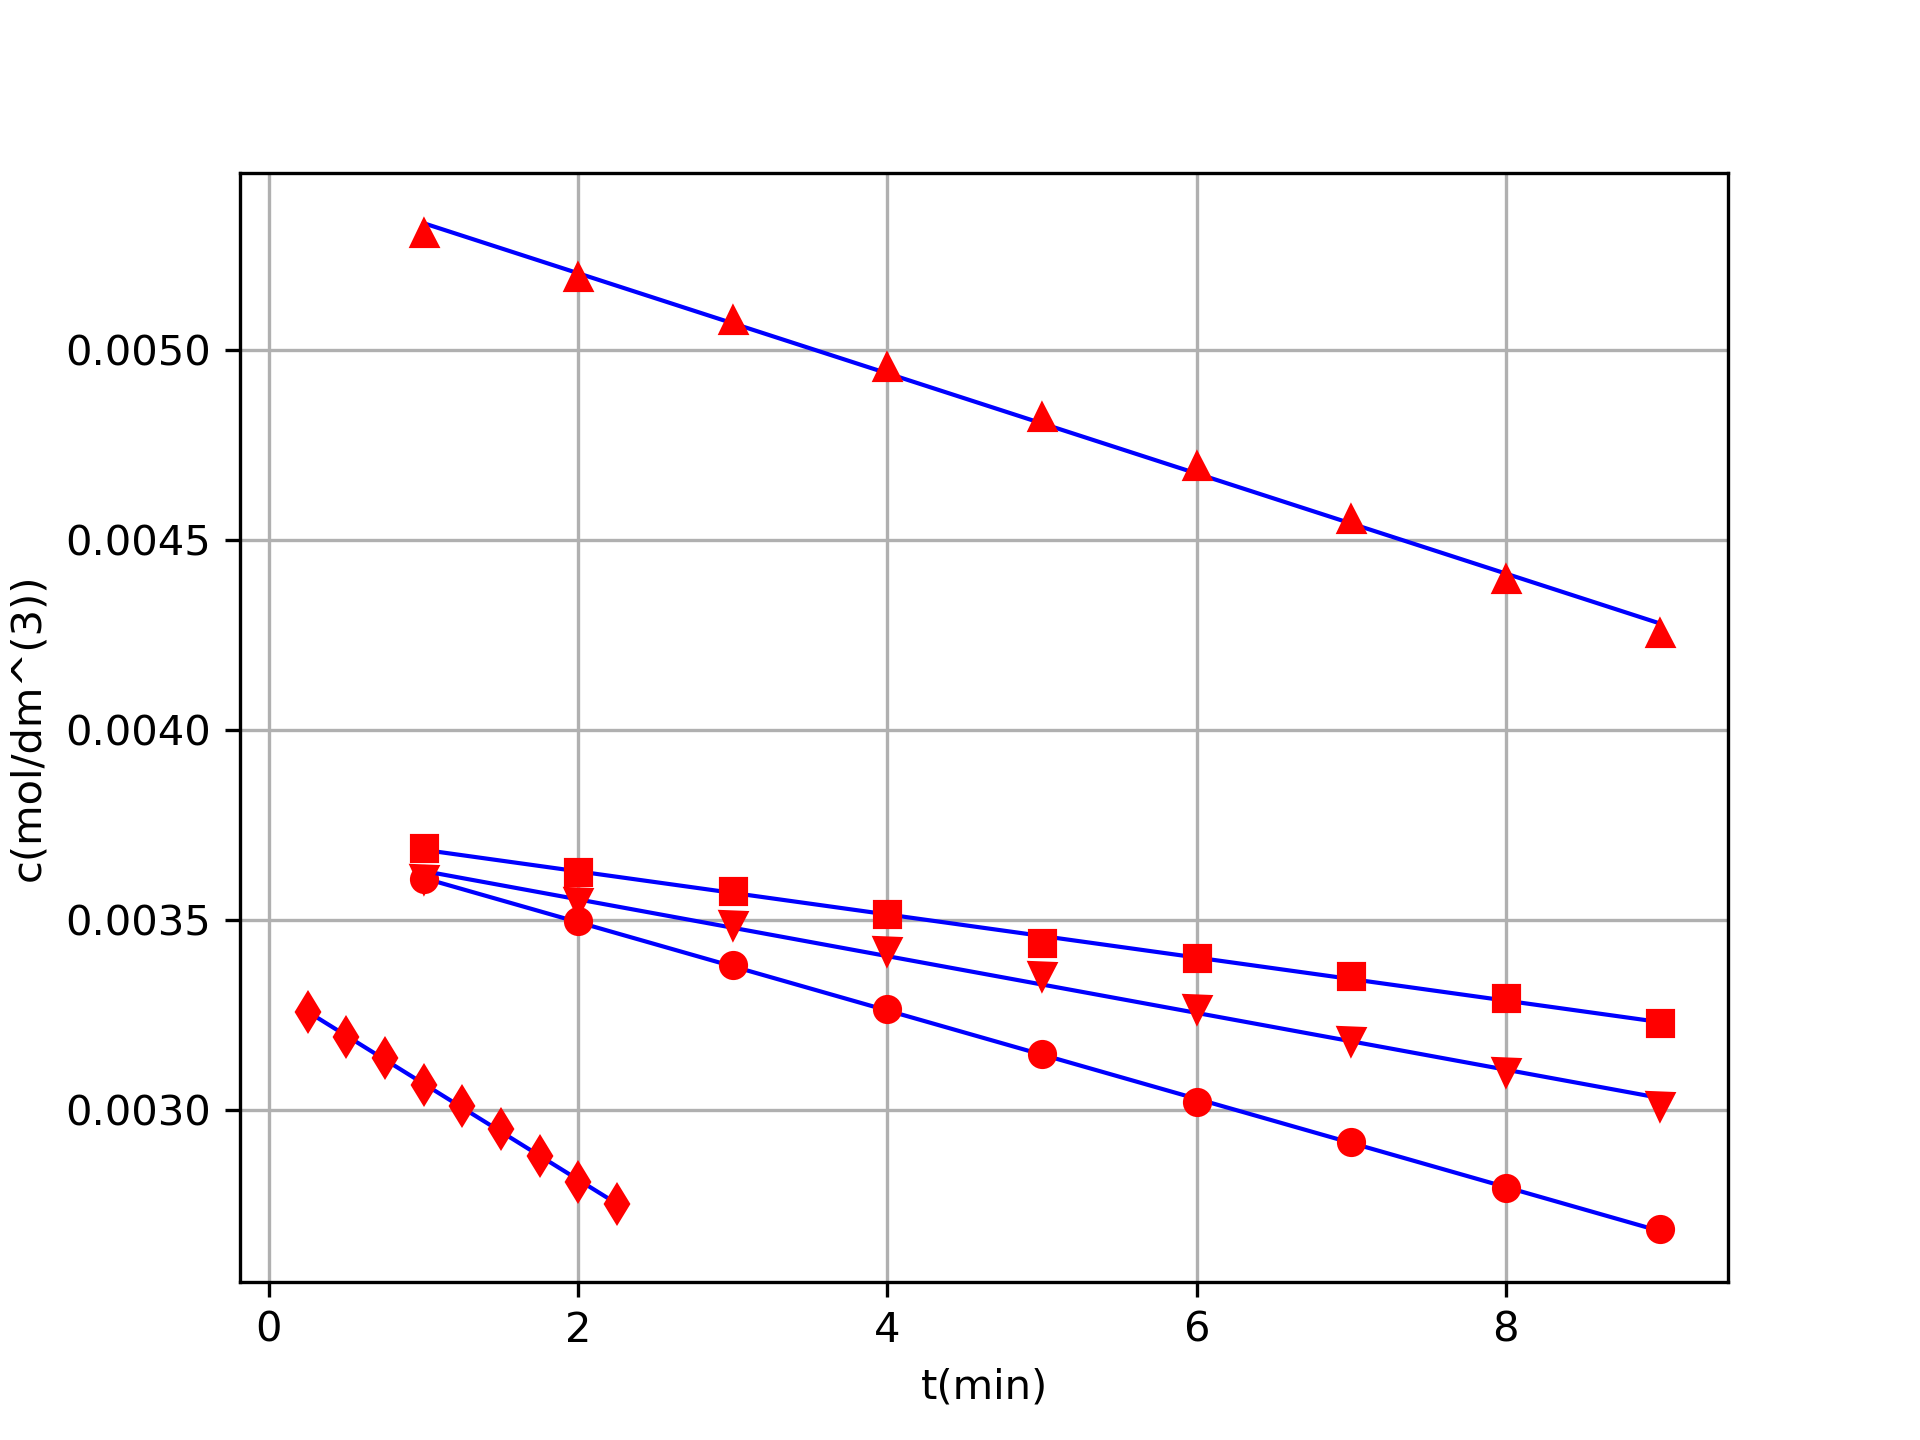
\includegraphics[width = .8\textwidth]{figures/result1.png}
\caption{线性拟合图像}
\label{fig:result1}
\end{figure}

\begin{figure}[H]
\centering
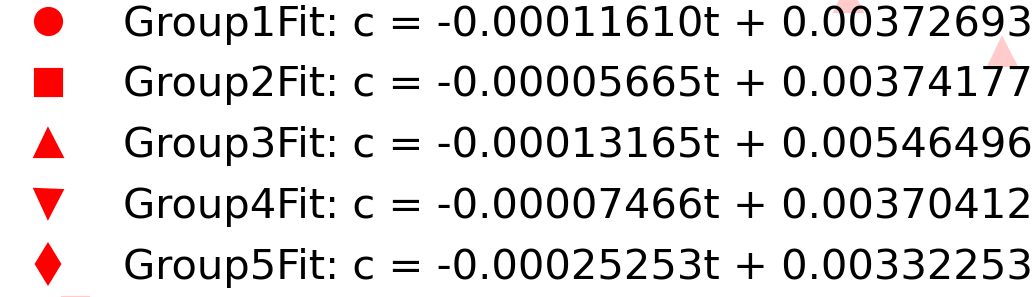
\includegraphics[width = .75\textwidth]{figures/result2.png}
\caption{线性拟合解析式}
\label{fig:result2}
\end{figure}
由于反应速率$r$即为上述拟合曲线斜率的负数,因此有(单位:mol/(L·min))
\begin{align*}
    r_1=1.16 \times 10^{-5}\\
    r_2=5.67 \times 10^{-6}\\
    r_3=1.32 \times 10^{-5}\\
    r_4=7.47 \times 10^{-6}\\
    r_5=2.53 \times 10^{-5} 
\end{align*}
\subsection{反应分级数计算}
由于反应中使用的是$0.02mol·dm^{-3}$碘溶液、$2.50mol·dm^{-3}$丙酮溶液和$1.00mol·dm^{-3}$盐酸溶液,根据表\ref{配比}的配比,可求得(单位均为mol/L)
\begin{align*}
    c_{\text{丙酮}}(1)=0.5\\
    c_{\text{丙酮}}(2)=0.25\\
    c_{\ce{I3^-}}(1)=4 \times 10^{-3}\\
    c_{\ce{I3^-}}(3)=6 \times 10^{-3}\\
    c_{H^+}(1)=0.2\\
    c_{H^+}(4)=0.1
\end{align*}
将上述数据代入以下公式,可以求得
\begin{equation}
\alpha=\frac{\ln r_1-\ln r_2}{\ln c_{\text {丙酮 }}(1)-\ln c_{\text {丙酮 }}(2)}=1.03
\label{eq:alpha}
\end{equation}
\begin{equation}
\beta=\frac{\ln r_1-\ln r_3}{\ln c_{\ce{I3^-}}(1)-\ln c_{\ce{I3^-}}(3)}=0.32
\label{eq:beta}
\end{equation}

\begin{equation}
\gamma=\frac{\ln r_1-\ln r_4}{\ln c_{\mathrm{H}^{+}}(1)-\ln c_{\mathrm{H}^{+}}(4)}=0.63
\label{eq:gamma}
\end{equation}

\subsection{反应速率系数和表观活化能计算}
\subsubsection{25℃下反应速率系数}
    25℃下反应速率系数的计算如表\ref{tab:k1_cal}所示(单位均为mol/L)。
\begin{table}[H]
\centering
\caption{25℃下反应速率系数计算}
\label{tab:k1_cal}
\begin{tabularx}{0.85\textwidth}{ccccccccc}
\toprule
编号 & $c_{\text{丙酮}}$ & $c_{\text{丙酮}}^\alpha$ & $c_{\ce{I3^-}}$ & $c_{\ce{I3^-}}^\beta$ & $c_{\mathrm{H}^{+}}$ & $c_{\mathrm{H}^{+}}^\gamma$ & $r$ & $k$ \\
\midrule
1 & 0.5 & 0.4897 & 0.004 & 0.1709 & 0.2 & 0.3628 & $1.26\times 10^{-5}$ & $4.15\times 10^{-4}$ \\
2 & 0.25 & 0.2398 & 0.004 & 0.1709 & 0.2 & 0.3628 & $5.67\times 10^{-6}$ & $3.81\times 10^{-4}$ \\
3 & 0.5 & 0.4897 & 0.006 & 0.1945 & 0.2 & 0.3628 & $1.32\times 10^{-5}$ & $3.82\times 10^{-4}$ \\
4 & 0.5 & 0.4897 & 0.004 & 0.1709 & 0.1 & 0.2344 & $7.47\times 10^{-6}$ & $3.81\times 10^{-4}$ \\
\midrule
\multicolumn{8}{c}{平均} & $3.89\times 10^{-4}$ \\
\bottomrule
\end{tabularx}
\end{table}
若以秒为时间单位,则$k=6.48\times 10^{-6}$
\subsubsection{35℃下反应速率系数}
    
将表\ref{tab:k1_cal}第一组的浓度数据和35℃下$r_5=2.53 \times 10^{-5}$代入速率方程,可求得

$
k=8.33 \times 10^{-4}
$
若以秒为时间单位,则$k=1.39\times 10^{-5}$
\subsubsection{表观活化能}    
\begin{equation}
E_{\mathrm{a}}=\frac{R T_1 T_2}{T_2-T_1} \ln \frac{k_2}{k_1}=51.4kJ
\end{equation}
结果为负,大概率是35℃下透光率测量不准,导致35℃时反应速率系数小于25℃,以下会进行误差分析。
\section{结果与讨论}
\subsection{数据分析与讨论}



查阅数据得
$
    \alpha=0.939 \
    \beta=0.32 \
    \gamma = 0.989 \
$
比较自己算得的
$
    \alpha=1.03\
    \beta=0.32\
    \gamma = 0.63\
$
可以发现$\alpha$结果相近,说明第一组和第二组数据在测定时操作准确,结果接近真实值。$\beta$偏大,相对误差很大,而$\gamma$偏小,且测定误差较大。

$\beta$的实际值应为零,则实验中由第三组数据测得的反应速率$r_3$偏大,$r_3$理应和$r_1$接近。$\gamma$值偏小,说明反应中$r_4$值偏大。

我认为以上的误差可能是由如下因素造成的:
 两组测定开始前,待测液配制时间长度不一,导致开始测定时反应进度不同。观察第一组和第三组实验,理论是该反应是碘的零级反应,在其他物质配比保持一定时,改变碘的浓度并不会改变反应的速率,而实验结果表明,两者速率并没有完全一致,这很可能就是操作上的细小误差导致结果的天差地别;配制溶液前要充分清洗容量瓶,每次操作完要用去离子水充分清洗比色皿并将比色皿光面擦拭干净,这些操作如果没有仔细进行也会给实验结果带来误差;还有可能是丙酮标准溶液由于多次倾倒,丙酮挥发,浓度并非是标定浓度,这也会给结果带来较大误差。


查阅资料得丙酮碘化反应25℃时速率常数为$5.38 \times 10^{-6}$,同时其指出通常丙酮酸反应速率常数的数量级是$10^{-6}$或$10^{-6}$。实验计算得到的k为$6.48 \times 10^{-6}$,相对误差为20.4\%,测得的速率常数在量级上无误,但是仍然存在误差,我认为其中主要原因是由于在实验过程中恒温水域箱出现故障,不能准确控制水域温度,反应体系并非是在恒温25摄氏度进行的,第三组、第二组水域温度达到了27.9摄氏度。

\subsection{总结与反思}

本次实验通过分光光度法测定了丙酮碘化反应中透光率随时间的变化,利用朗伯比耳定律确定了碘浓度的变化,并进一步计算了反应速率。采用孤立系数法得出了反应的反应级数、速率系数以及表观活化能。实验过程中要求操作严谨,精确性要求较高,对仪器设备的准确性也有一定要求。实验中出现的失误情况经过分析,并对实验操作提出了改进方案,以提高实验的准确性和可重复性。通过对误差的分析,对实验原理有了更深刻的理解和认识。

这次实验通过数据处理的到的结果误差较大,然而实验过程中并没有比较明显的操作失误,可见原始数据细小的误差也很可能会使实验结果大相径庭,所以之后的实验中任何已经重复过无数次的操作,例如用容量瓶标定溶液、测透光率等等操作都要多加注意,减少操作带来的实验误差,提高最后实验结果的准确度。


\section{思考题}
\subsection{动力学实验中,正确计算时间是很重要的。本实验中从反应物开始混合到起算反应时间,中间有一段不算很短的操作时间,这对实验结果有无影响?为什么?}
我认为是有影响的,在温度较高的情况下,反应进行的很快,如果没有操作迅速,可能导致测量还没有结束反应已经停止,这会导致数据点的减少,给实验结果带来误差。\\
此外,任何延迟或不准确的计时都可能导致最终结果的误差。特别是在动力学实验中,反应速率常数的准确测量对于确定反应机理和动力学性质至关重要。因此,确保准确的起始时间点和严格的时间测量是至关重要的,以减小时间误差对实验结果的影响。
\subsection{影响本实验结果的主要因素是什么?}
  \begin{itemize}
      \item 溶液浓度和配制准确性:在实验中,需要准确地量取和配制溶液,以保证实验结果的准确性。在配制待测溶液时不要忘记定容操作。
      \item 温度:实验温度需要保持恒定,以保证实验结果的可靠性。恒温箱温度应该略高于25℃,因为在恒温水通进分光光度计比色套的过程中水温会略有下降。
      \item 比色皿润洗和清洁:每次测量之前比色皿的光面需要保持清洁,同时每次使用前需要用待测液进行润洗,以避免影响透光率测定。

  \end{itemize}
  \subsection{设计确定丙酮溴化反应速率方程的实验步骤。}
    步骤如下:
    \begin{enumerate}
        \item 准备实验材料
        \item 制备反应混合物: 先标定溴化钾,再利用溴化钾和硫酸制备溴水(现配现用),随后标定溴水中的\ce{H^+}。在三个磨口瓶中分别加入已标定的丙酮,溴水和硫酸。
        \item 分光光度计校正:用去离子水校正分光光度计的透光率数值,并根据溴的吸收峰,测量已知浓度溴的透光率,求出$\varepsilon l$。
        \item 准备测量:按照孤立系数法的原理,依照一定的配比向容量瓶混合一定量的丙酮、溴化钾和硫酸,定容。确保混合物中的浓度是可控制的,并且在实验过程中可以进行变化,搅拌或振荡混合反应物。
        \item 开始反应:依照本实验的方法依次测定透光率。
        \item 数据处理
    \end{enumerate}

需要注意的是溴水必须现配现用,同时配制溴水时硫酸可能过量,因此还要标定溴水中的\ce{H^+},最终\ce{H^+}的配比需要综合考虑溴水和硫酸溶液。同时溴的特征吸收峰和碘不同,实验前需事先查阅。


\end{document}
